\chapter{Упражнения по работе с пользовательскими функциями \unf}

Освоить работу с расчетными функциями \unf можно выполняя упражнения описанные в данном разделе и изучая устройство тестовых расчетных модулей. Упражнение демонстрируют некоторые подходы к использованию \unf. На основе этих подходов можно создать свои расчетные модули решающие специфические задачи пользователя. 

\section{Расчет PVT свойств}

Расчет физико химических свойств пластовых флюидов лежит в основе всех расчетов систем нефтедобычи. При решении прикладных задач редко возникает необходимость расчета PVT свойств непосредственно, однако понимание принципа их расчета, а особенно зависимости результатов расчета от исходных данных важно.
	
Цель упражнений по расчету PVT свойств:
\begin{itemize}	
	\item 	освоить принципы работы c пользовательскими функций \unf 
	\item 	изучить влияние исходных PVT данных на результаты расчета PVT свойств
	\item 	изучить влияние выбора PVT корреляций на результаты расчета PVT свойств
	\item 	изучить механизм калибровки PVT корреляций на результаты измерений
\end{itemize}
	 
	 
\subsection{Построение простых PVT зависимостей}

Для выполнения упражнения используйте файл "10.PVT.xlsx"

\begin{enumerate}
	\item Запустите файл с надстройкой \unf. Для того чтобы убедиться, что надстройка запущена откройте редактор VBE (Alt+F11). В дереве проектов должен отображаться файл надстройки \mintinline{vb.net}{UniflocVBA_7.xlam}, рис. \ref{ris:VBE_empty}.
	
	\begin{figure}[h!]
		\center{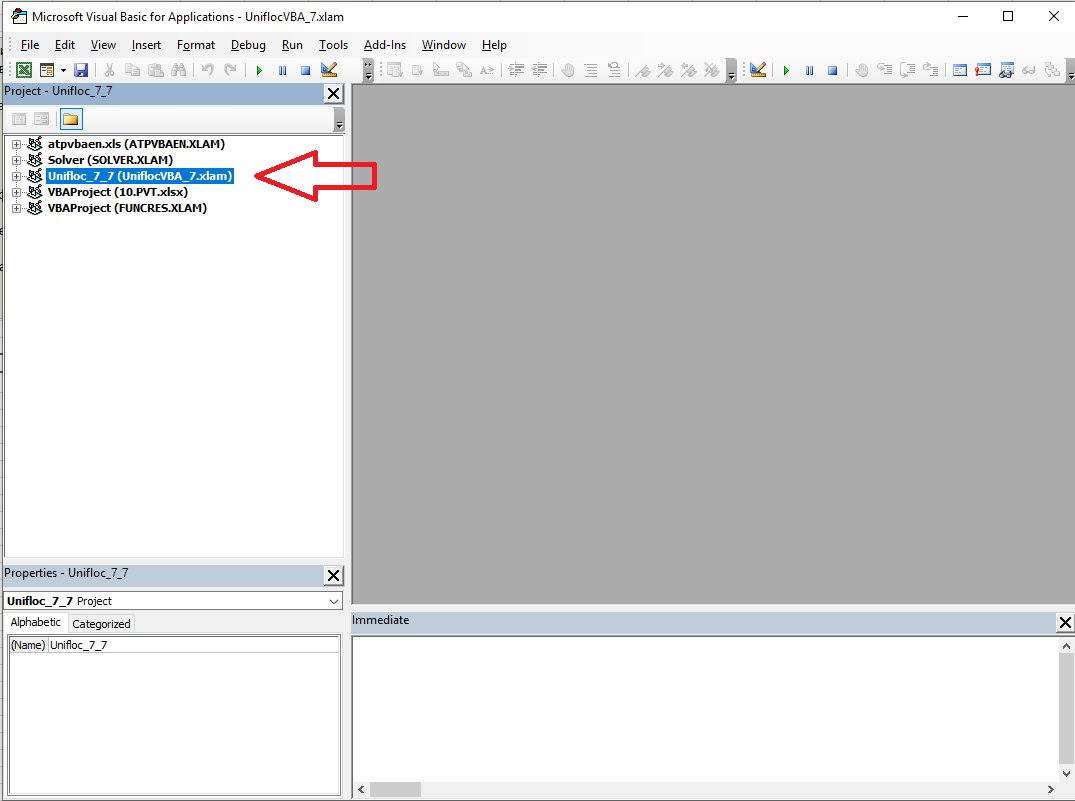
\includegraphics[width=0.5\linewidth]{VBE_empty}}
		\caption{Окно редактора VBE с загруженной надстройкой \unf}
		\label{ris:VBE_empty}
	\end{figure}

	\item Откройте файл с упражнением \texttt{10.PVT.xlsx} (смотри рис. \ref{ris:Ex10_1}).
	
	\begin{figure}[h!]
		\center{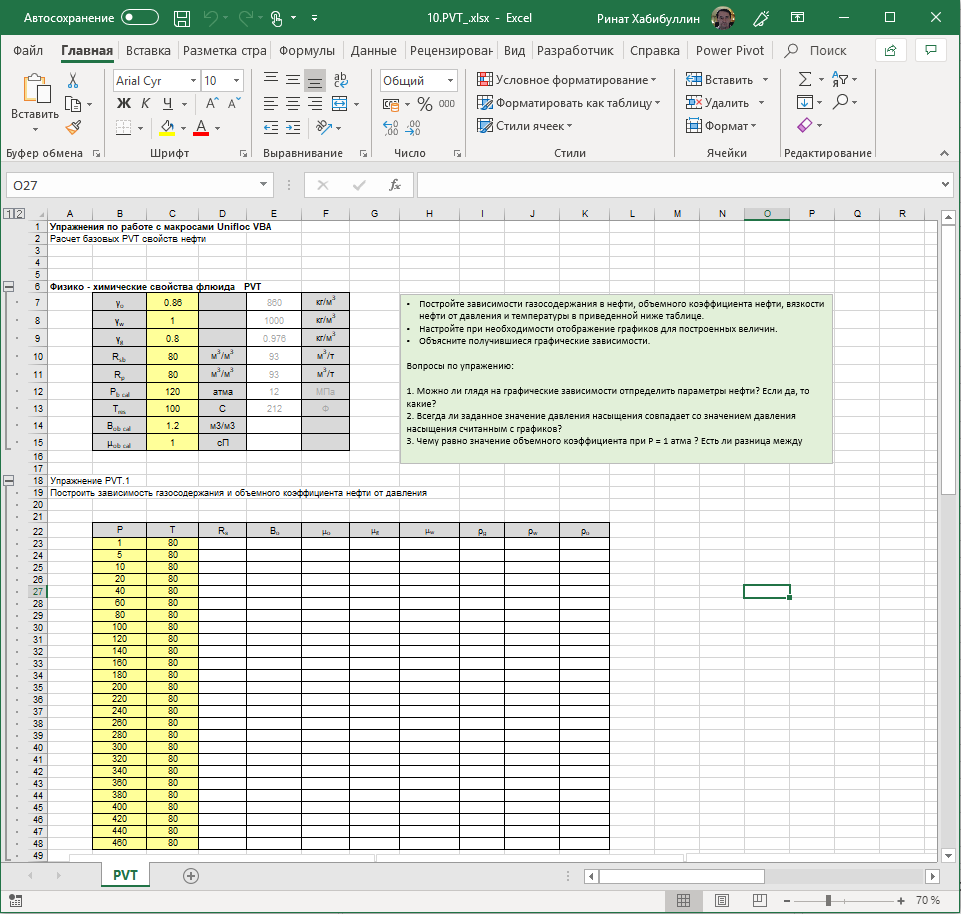
\includegraphics[width=0.5\linewidth]{Ex10_1}}
		\caption{Открытый файл с упражнением \texttt{10.PVT.xlsx}}
		\label{ris:Ex10_1}
	\end{figure}
	
	\item Для расчета первого элемента таблицы в ячейках D23:D48 - газосодержания в нефти при давлении 1 атм и температуре 80 °C - введите в ячейку D23 строку
	
	{ \small  \texttt{=PVT\_Rs\_m3m3(B23;C23;gamma\_gas\_;gamma\_oil\_; gamma\_wat\_; Rsb\_; Rp\_; Pb\_; Tres\_; Bob\_; muob\_)}}
	
	Обратите внимание -- при запущенной надстройке достаточно начать вводить в ячейку формулу, например ввести \texttt{=PVT} как Excel откроет выпадающий список с подсказкой, показывающий возможные варианты названий функций (смотри рис. \ref{ris:Ex10_2}). 
	
	В приведенной строке \texttt{B23;C23} - ссылки на соответствующие ячейки,  \texttt{gamma\_gas\_;gamma\_oil\_} - также ссылки на ячейки, которые предварительно были поименованы. 

	\begin{figure}[h!]
		\center{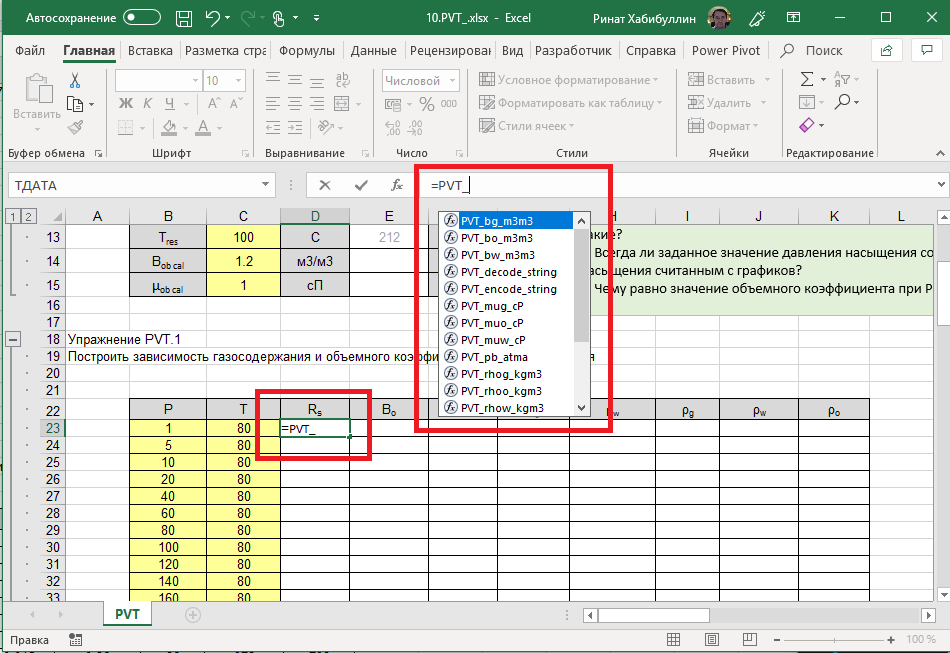
\includegraphics[width=0.5\linewidth]{Ex10_2}}
		\caption{Выпадающий список с подсказками названий функции}
		\label{ris:Ex10_2}
	\end{figure}

	Из выпадающего списка выберите функцию \texttt{=PVT\_Rs\_m3m3(} после чего нажмите кнопку $f_x$ "вставить функцию"  слева от строки формул. Это вызовет окно задания параметров функции, в котором будут указаны все параметры, которые необходимо ввести. В этом окно можно ввести необходимые значения параметров или указать ссылки на соответствующие ячейки.

	\begin{figure}[h!]
		\center{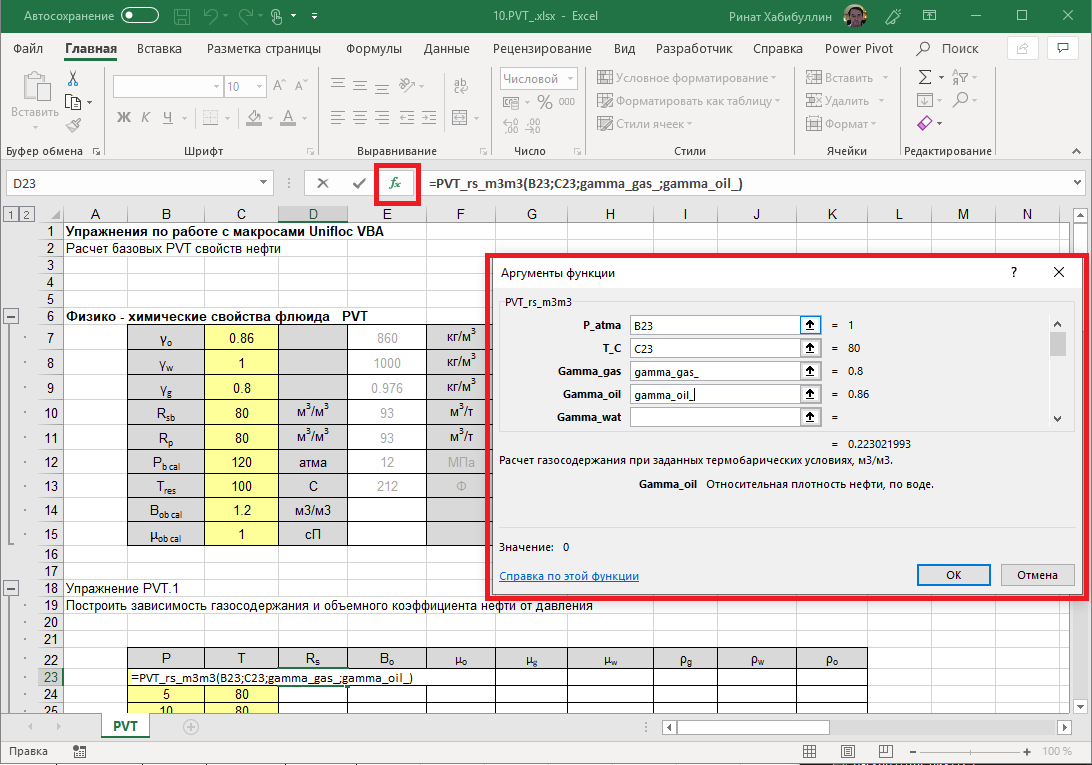
\includegraphics[width=0.5\linewidth]{Ex10_3}}
		\caption{Окно ввода аргументов функции}
		\label{ris:Ex10_3}
	\end{figure}

	\item После ввода всех параметров и нажатия кнопки ОК в ячейке должен отобразиться результат расчета. Воспользовавшись инструментом "Влияющие ячейки" на вкладке "Формулы" можно отследить на какие ячейки ссылается введенная формула
	\begin{figure}[h!]
		\center{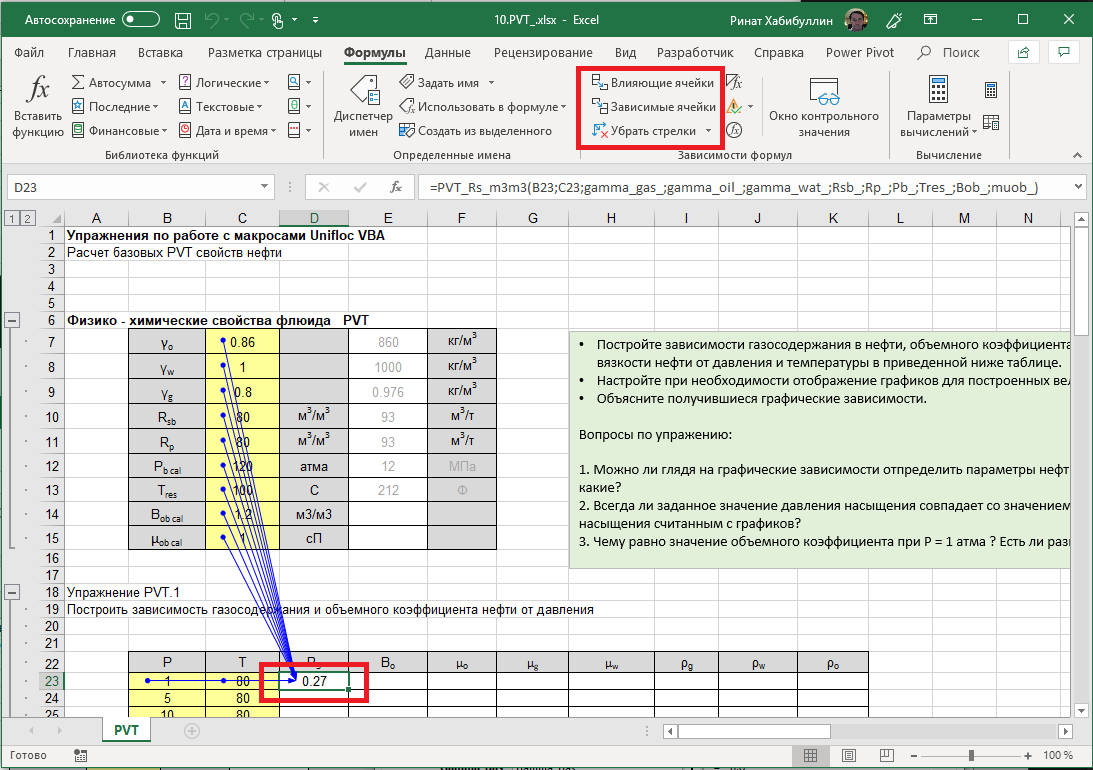
\includegraphics[width=0.5\linewidth]{Ex10_4}}
		\caption{Результат вызова пользовательской функции с отображение влияющих ячеек}
		\label{ris:Ex10_4}
	\end{figure}

	\item Аналогично заполните все ячейки таблицы  \texttt{D23:D48} вызовами функции \texttt{=PVT\_Rs\_m3m3()} с соответствующими параметрами. Это можно сделать "протянув" ранее введенную функцию в ячейке \texttt{D23}.
	
	Обратите внимание, что при "протягивании" поименованные ячейки оказываются закрепленными, а ссылки на значения давления и температуры съезжают вместе с протягиваемой ячейкой. Результат показан на рисунке \ref{ris:Ex10_5}
	\begin{figure}[h!]
		\center{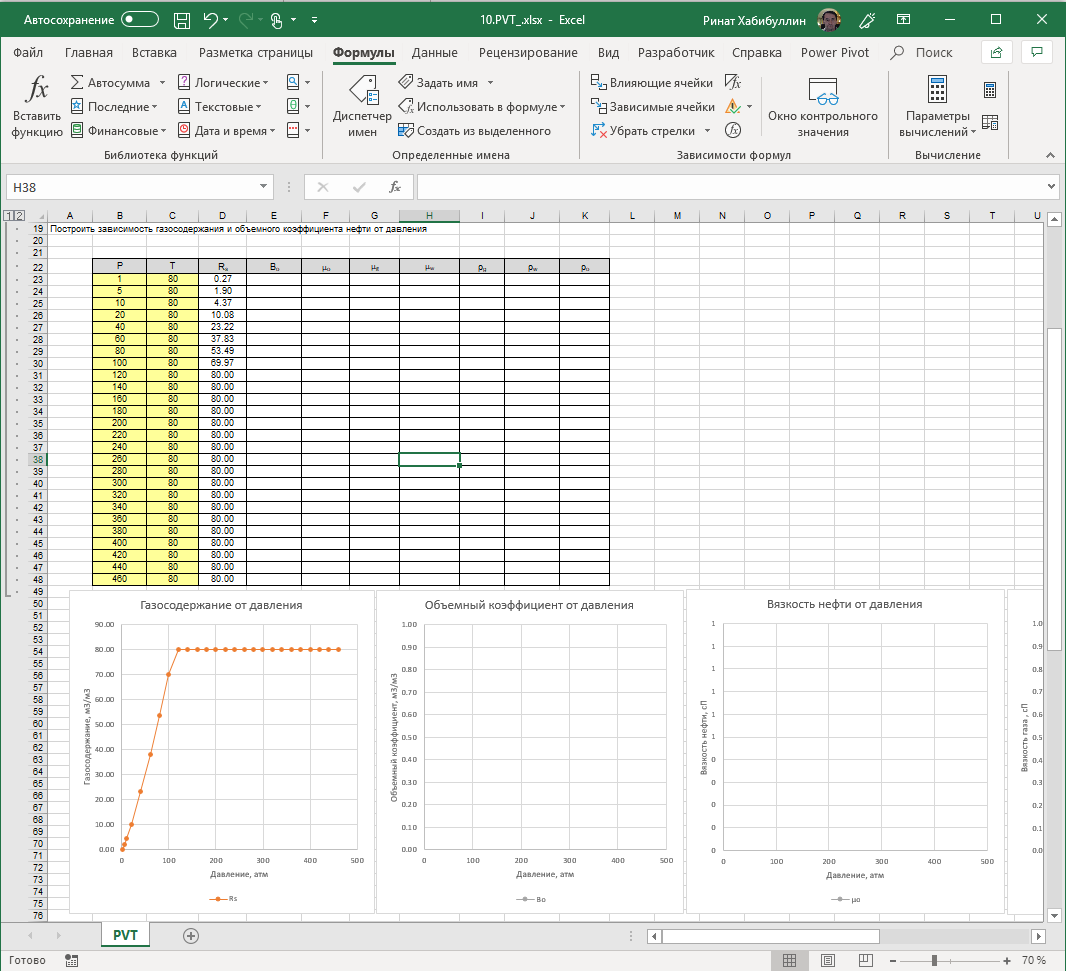
\includegraphics[width=0.5\linewidth]{Ex10_5}}
		\caption{Результат расчета зависимости газосодержания от давления}
		\label{ris:Ex10_5}
	\end{figure}

	\item По аналогии с зависимостью газосодержания от давления постройте графики зависимости других параметров от давления. Используйте следующие функции для проведения расчатов: 
	
	функция расчета объемного коэффициента нефти
	
	{ \small  \texttt{=PVT\_Bo\_m3m3(B23;C23;gamma\_gas\_;gamma\_oil\_;gamma\_wat\_; Rsb\_; Rp\_; Pb\_;Tres\_;Bob\_;muob\_)}}
	
	функция расчета вязкости нефти при заданных термобарических условиях
	
	{ \small  \texttt{=PVT\_Muo\_cP(B23;C23;gamma\_gas\_;gamma\_oil\_;gamma\_wat\_; Rsb\_; Rp\_; Pb\_;Tres\_;Bob\_;muob\_)}}
	
    функция расчета вязкости газа при заданных термобарических условиях
	
	{ \small  \texttt{=PVT\_Mug\_cP(B23;C23;gamma\_gas\_;gamma\_oil\_;gamma\_wat\_; Rsb\_; Rp\_; Pb\_;Pb\_;Bob\_;muob\_)}}
	
	функция расчета вязкости воды при заданных термобарических условиях
	
	{ \small  \texttt{=PVT\_Muw\_cP(B23;C23;gamma\_gas\_;gamma\_oil\_;gamma\_wat\_; Rsb\_; Rp\_; Pb\_;Tres\_;Bob\_;muob\_)}}
	
	функция расчета плотности газа при заданных термобарических условиях
	
	{ \small  \texttt{=PVT\_Rhog\_kgm3(B23;C23;gamma\_gas\_;gamma\_oil\_;gamma\_wat\_; Rsb\_; Rp\_; Pb\_;Tres\_;Bob\_;muob\_)}}
	
	функция расчета плотности воды при заданных термобарических условиях
	
	{ \small  \texttt{=PVT\_Rhow\_kgm3(B23;C23;gamma\_gas\_;gamma\_oil\_;gamma\_wat\_; Rsb\_; Rp\_; Pb\_;Tres\_;Bob\_;muob\_)}}
	
	функция расчета плотности нефти при заданных термобарических условиях
	
	{ \small  \texttt{=PVT\_Rhoo\_kgm3(B23;C23;gamma\_gas\_;gamma\_oil\_;gamma\_wat\_; Rsb\_; Rp\_; Pb\_;Tres\_;Bob\_;muob\_)}}
	
	Результаты приведены на рисунке \ref{ris:Ex10_6}
	
	\begin{figure}[h!]
		\center{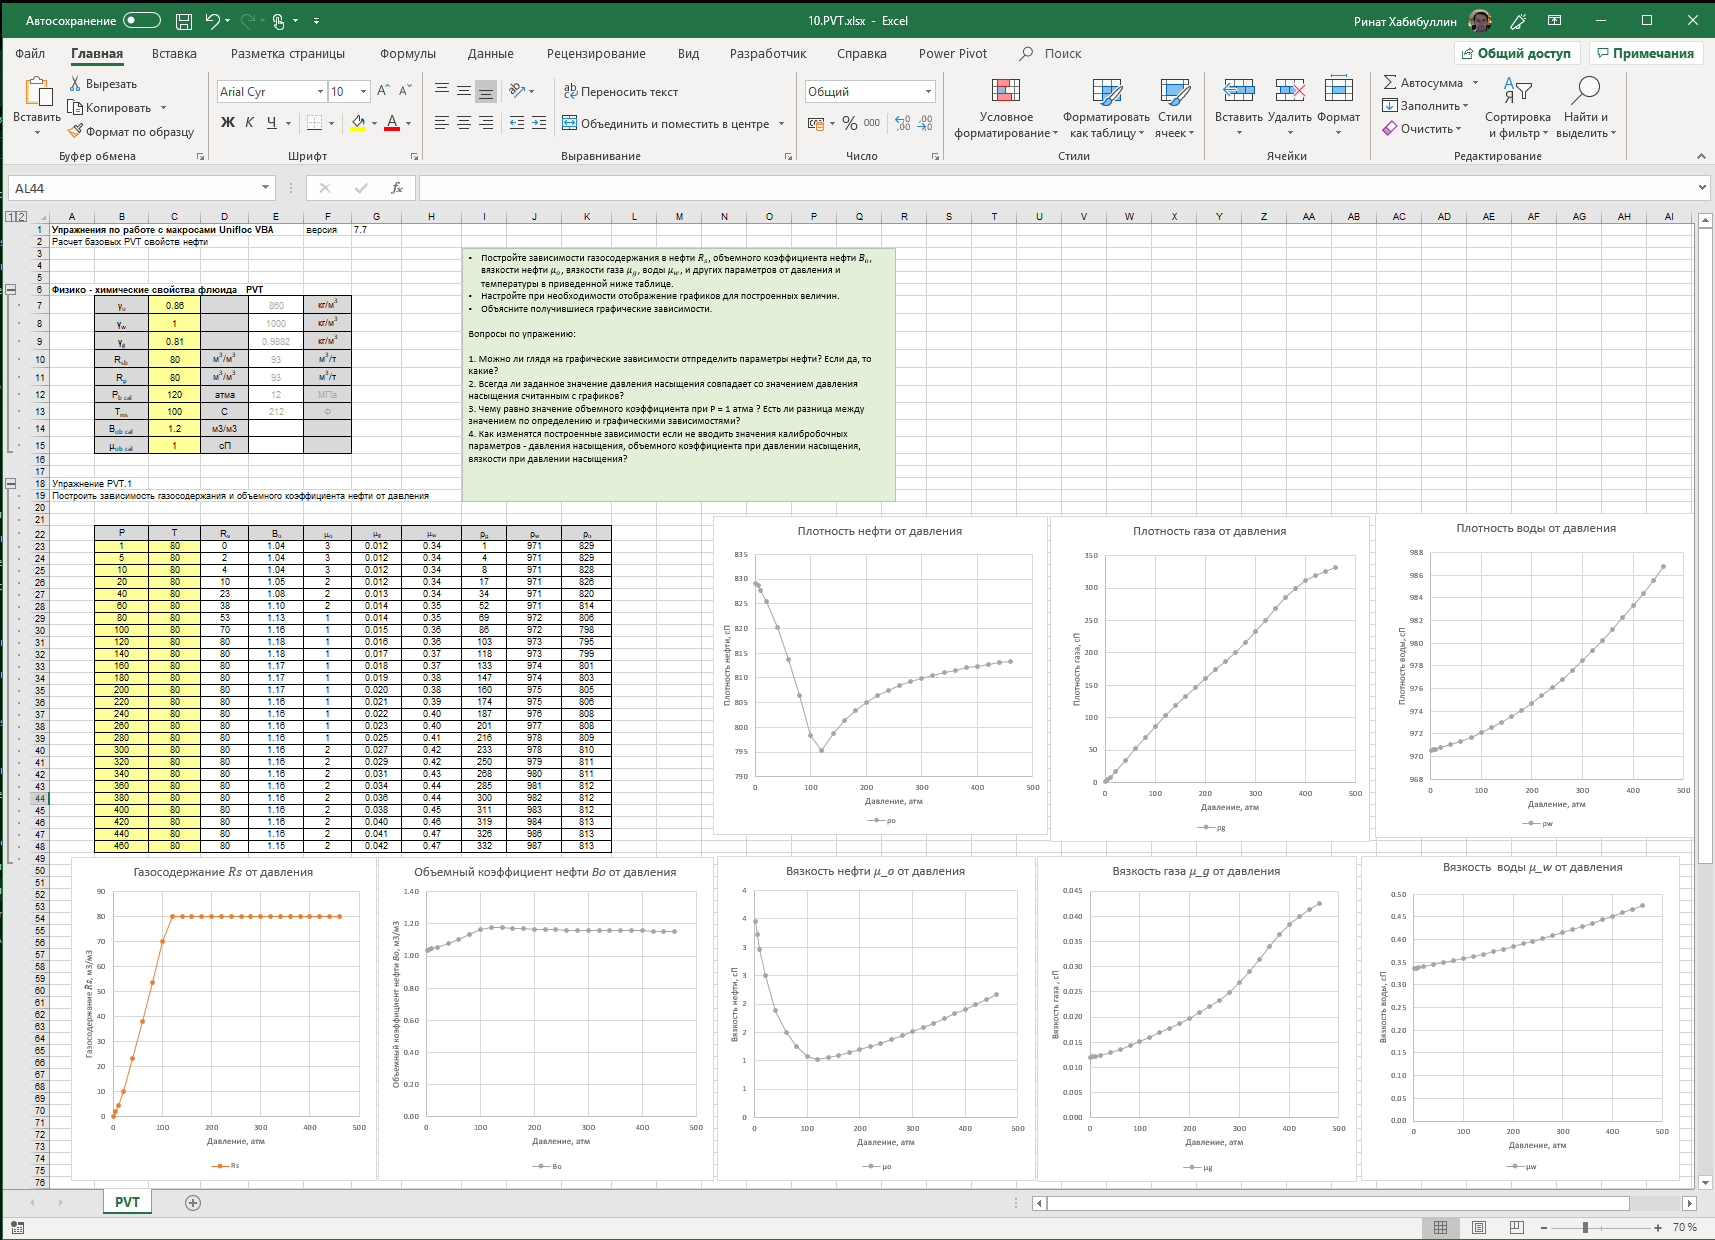
\includegraphics[width=1\linewidth]{Ex10_6}}
		\caption{Результат расчета зависимости свойств пластовых флюидов от давления}
		\label{ris:Ex10_6}
	\end{figure}
	
	\item Ответьте на вопросы по упражнению приведенные в рабочей книге.
	
	\begin{enumerate}
		\item Можно ли глядя на графические зависимости определить параметры нефти? Если да, то какие?
		\item Всегда ли заданное значение давления насыщения совпадает со значением давления насыщения считанным с графиков?
		\item Чему равно значение объемного коэффициента при Р = 1 атма? Есть ли разница между исходным значением и значением определенным по графическими зависимостями?
		\item Как изменятся построенные зависимости если не вводить значения калибровочных параметров - давления насыщения, объемного коэффициента при давлении насыщения, вязкости при давлении насыщения?
		
	\end{enumerate}
 
\end{enumerate}

\section{Расчет производительности скважины}

Модель притока к скважине является достаточно простой и одновременно полезной, позволяя оперативно оценивать добычные возможности скважины. Для индикаторной диаграммы Вогеля зависимость забойного давления от дебита ниже давления насыщения перестает быть линейной.

Для выполнения упражнения необходимо задать:
\begin{enumerate}
	\item PVT свойства флюидов
	\item Параметры работы скважины на установившемся режиме
	\item Пластовое давление
\end{enumerate}


\begin{figure}[h!]
	\center{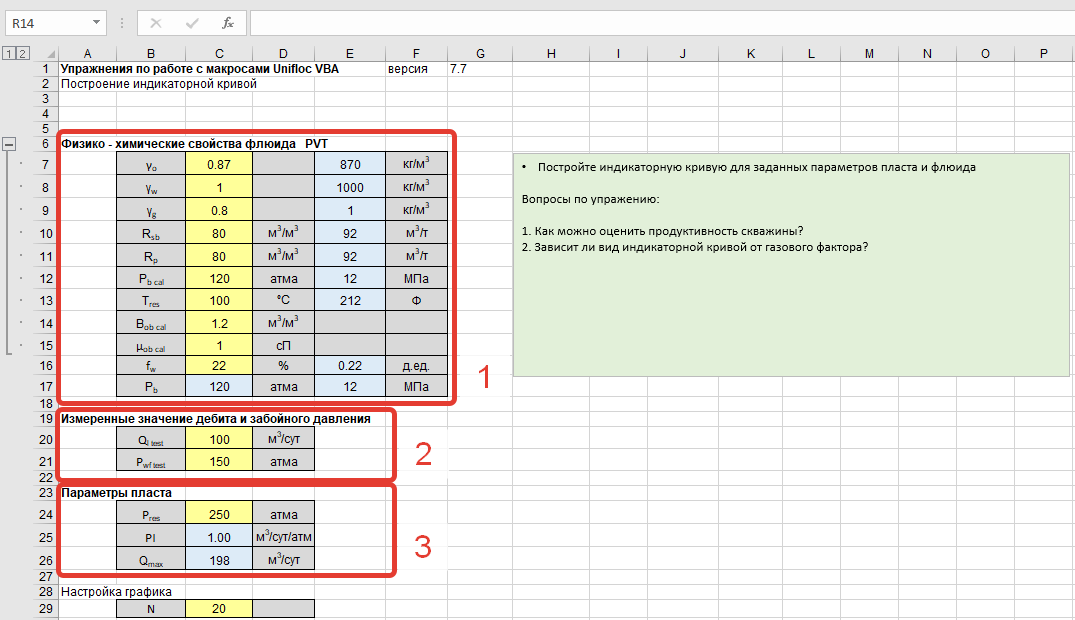
\includegraphics[width=1\linewidth]{Ex20_1}}
	\caption{Исходные данные для построения индикаторной кривой}
	\label{ris:Ex20_1}
\end{figure}

Коэффициент продуктивности $PI$ скважины рассчитывается в ячейке С25 по замеренным данным  с помощью функции

{ \small  \texttt{=IPR\_PI\_sm3dayatm(qltest\_;Pwftest\_;Pres\_;fw\_;Pb\_)}}

А максимальный дебит $Q_{max}$ при максимальной депрессии с забойным давлением равным нулю

{ \small  \texttt{=IPR\_Qliq\_sm3Day(PI\_;Pres\_;0;fw\_;Pb\_)}}

После задания всех необходимых параметров перейдем к построению индикаторной кривой.

Для расчета забойного давления в зависимости от дебита введите в ячейку D40 строку

{ \small  \texttt{=IPR\_Pwf\_atma(PI\_;Pres\_;C40;fw\_;Pb\_)}}

Для вычисления дебита в зависимости от давления Вы можете воспользоваться функцией 

{ \small  \texttt{=IPR\_Qliq\_sm3Day(PI\_;Pres\_;D40;fw\_;Pb\_)}}

поместив ее в ячейку E40.

\begin{figure}[h!]
	\center{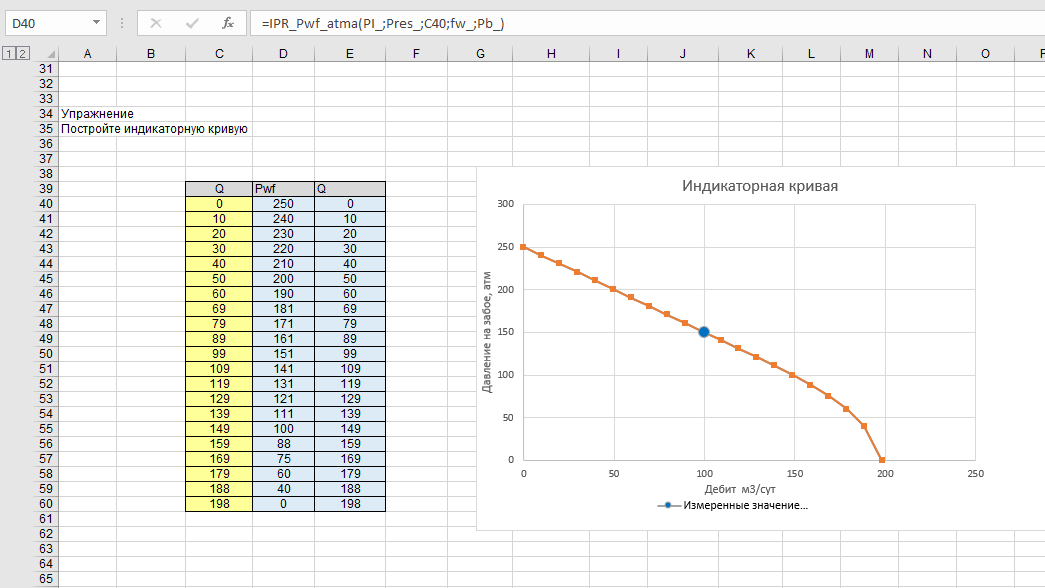
\includegraphics[width=1\linewidth]{Ex20_2}}
	\caption{Результат построения индикаторной кривой}
	\label{ris:Ex20_2}
\end{figure}

Применяя функции, строя дополнительные графики, ответьте на вопросы по упражнению, приведенные в рабочей книге.

	\begin{enumerate}
		\item Как можно оценить продуктивность скважины?
		\item Зависит ли вид индикаторной кривой от газового фактора?
	\end{enumerate}



\section{Расчет свойств многофазного потока}

Расчет характеристики потока, состоящего из двух или более фаз, является более сложным, чем вычисление параметров однофазного потока. Вследствие разности плотностей и вязкостей, поведение фаз в потоке может существенно различаться. Расчет параметров газожидкостной смеси необходим для прогнозирования распределения давления в скважине, анализа работы погружного оборудования и т.д.
 
Аналогично предыдущим упражнениям сперва необходимо задать:
	\begin{enumerate}
		\item PVT свойства флюидов
		\item Параметры потока флюида - $Q_{l}$ - расход жидкости и $f_{w}$ - обводненность.
	\end{enumerate}
После этого в ячейке С20 для удобства использования все PVT свойства сгруппируются в единую строку с помощью функции

{ \small  \texttt{=PVT\_encode\_string(gamma\_gas\_;gamma\_oil\_;gamma\_wat\_;Rsb\_;Rp\_;Pb\_;Tres\_;Bob\_;muob\_)}}

\begin{figure}[h!]
	\center{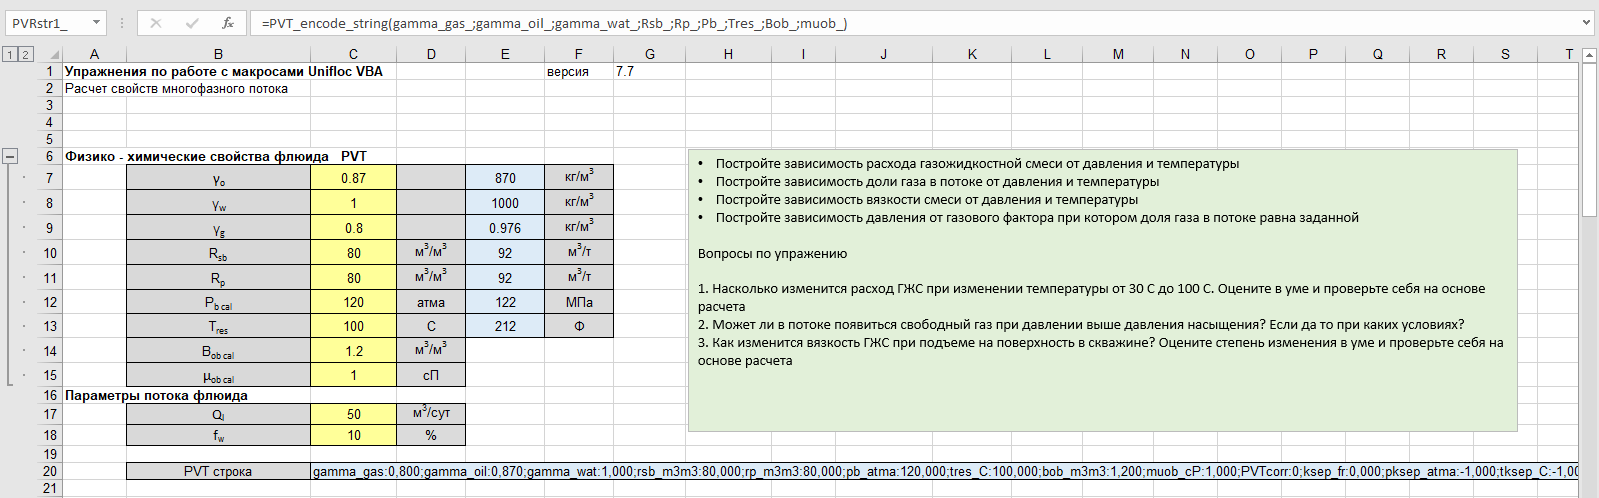
\includegraphics[width=1\linewidth]{Ex30_1}}
	\caption{Исходные данные для расчета параметров многофазного потока}
	\label{ris:Ex30_1}
\end{figure}

Для расчета параметров смеси при разных термобарических условиях вставьте следующие функции в таблицу и "протяните"\ их для полного заполнения.

Для расчета $Q_{mix}$ - объемного расхода смеси воспользуйтесь в ячейке E28 функцией

{ \small  \texttt{=MF\_Qmix\_m3day(Q\_;fw\_;C28;D28;PVRstr1\_)}}

Вычисление $\beta_{gas}$ - объемной доли газа в потоке в ячейке F28 производится с помощью функции

{ \small  \texttt{=MF\_gas\_fraction\_d(C28;D28;fw\_;PVRstr1\_)}}

А вязкости газожидкостной смеси $\mu_{mix}$ в G28

{ \small  \texttt{=MF\_Mumix\_cP(Q\_;fw\_;C28;D28;PVRstr1\_)}}

\begin{figure}[h!]
	\center{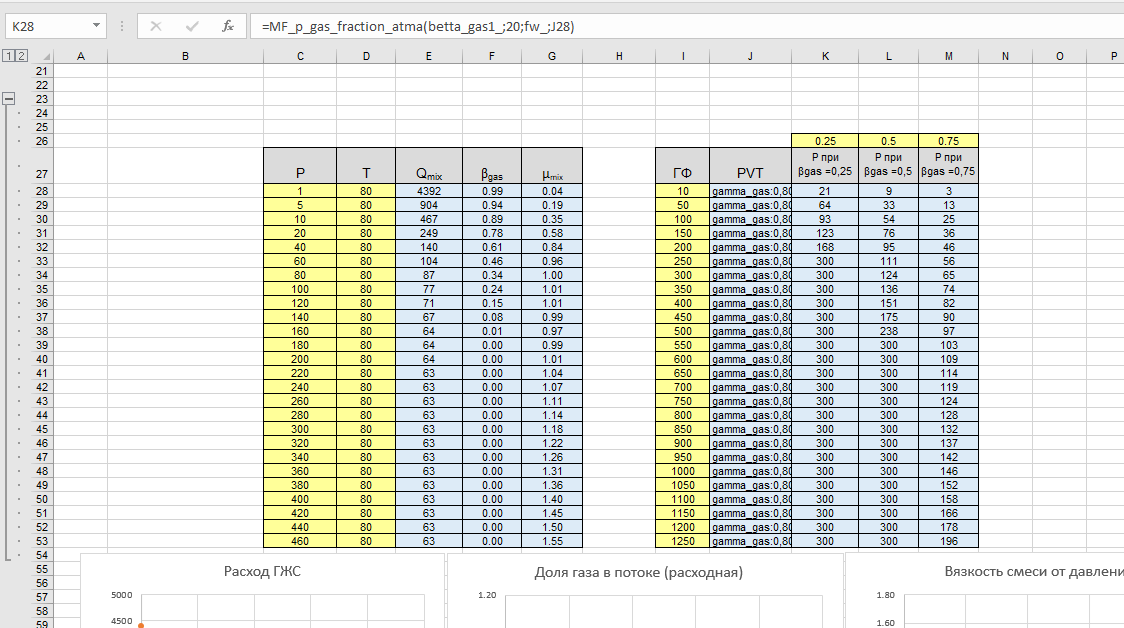
\includegraphics[width=1\linewidth]{Ex30_2}}
	\caption{Расчет параметров многофазного потока}
	\label{ris:Ex30_2}
\end{figure}

Для вычисления давления в зависимости от газового фактора и объемного содержания газа в потоке $\beta_{gas}$

Поместите в ячейку J28 строку:

{ \small  \texttt{=PVT\_encode\_string(gamma\_gas\_;gamma\_oil\_;gamma\_wat\_;Rsb\_;I28;Pb\_;Tres\_;Bob\_;muob\_)}}

А в ячейки K28, L28, M28 функцию для вычисления давления 

{ \small  \texttt{=MF\_p\_gas\_fraction\_atma(X;20;fw\_;J28)}}

где X соответствующие ссылки на ячейки с $\beta_{gas}$ - K26, L26, M26

\begin{figure}[h!]
	\center{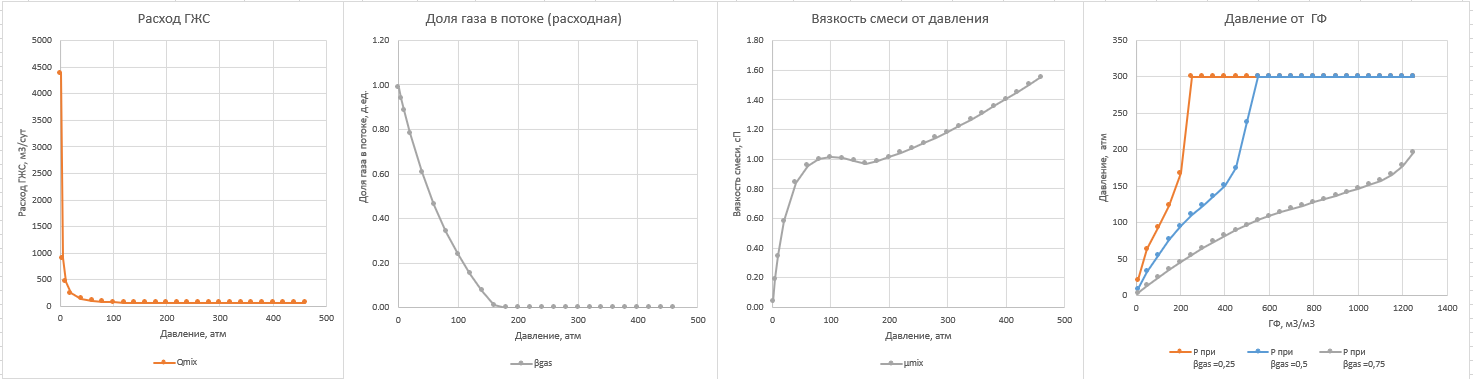
\includegraphics[width=1\linewidth]{Ex30_3}}
	\caption{Графики для параметров многофазного потока}
	\label{ris:Ex30_3}
\end{figure}

Далее для расчета вязкости отдельных фаз потока при различных P,T аналогично воспользуйтесь функциями.

Вязкость смеси $\mu_{mix}$ в E98

{ \small  \texttt{=MF\_Mumix\_cP(Q\_;fw\_;C98;D98;PVRstr1\_)}}

Вязкость газа $\mu_{gas}$ в F98

{ \small  \texttt{=PVT\_Mug\_cP(C98;D98;gamma\_gas\_;gamma\_oil\_;gamma\_wat\_;Rsb\_;Rp\_;Pb\_;Tres\_;Bob\_;muob\_)}}

Вязкость нефти $\mu_{o}$ в G98

{ \small  \texttt{=PVT\_Muo\_cP(C98;D98;gamma\_gas\_;gamma\_oil\_;gamma\_wat\_;Rsb\_;Rp\_;Pb\_;Tres\_;Bob\_;muob\_)}}

И вязкость воды $\mu_{w}$ в H98

{ \small  \texttt{=PVT\_Muw\_cP(C98;D98;gamma\_gas\_;gamma\_oil\_;gamma\_wat\_;Rsb\_;Rp\_;Pb\_;Tres\_;Bob\_;muob\_)}}

\begin{figure}[h!]
	\center{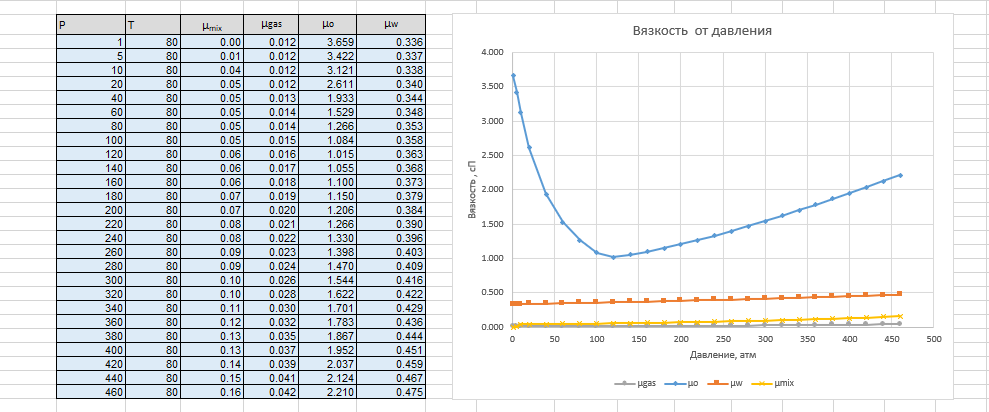
\includegraphics[width=1\linewidth]{Ex30_4}}
	\caption{Разложение вязкости смеси на отдельные компоненты}
	\label{ris:Ex30_4}
\end{figure}

Для самопроверки ответьте на следующие вопросы

\begin{enumerate}
	\item Насколько изменится расход ГЖС при изменении температуры от 30 С до 100 С? Оцените в уме и проверьте себя на основе расчета
	\item Может ли в потоке появиться свободный газ при давлении выше давления насыщения? Если да то при каких условиях?
	\item Как изменится вязкость ГЖС при подъеме на поверхность в скважине? Оцените степень изменения в уме и проверьте себя на основе расчета
\end{enumerate}


\section{Расчет штуцера}

Для контроля дебита и/или давления на добывающих скважинах вблизи устья может устанавливаться штуцер.

Расчет потока через данное гидравлическое сопротивление начинается с предварительного задания PVT свойств, параметров потока и конструкции элементов.

\begin{figure}[h!]
	\center{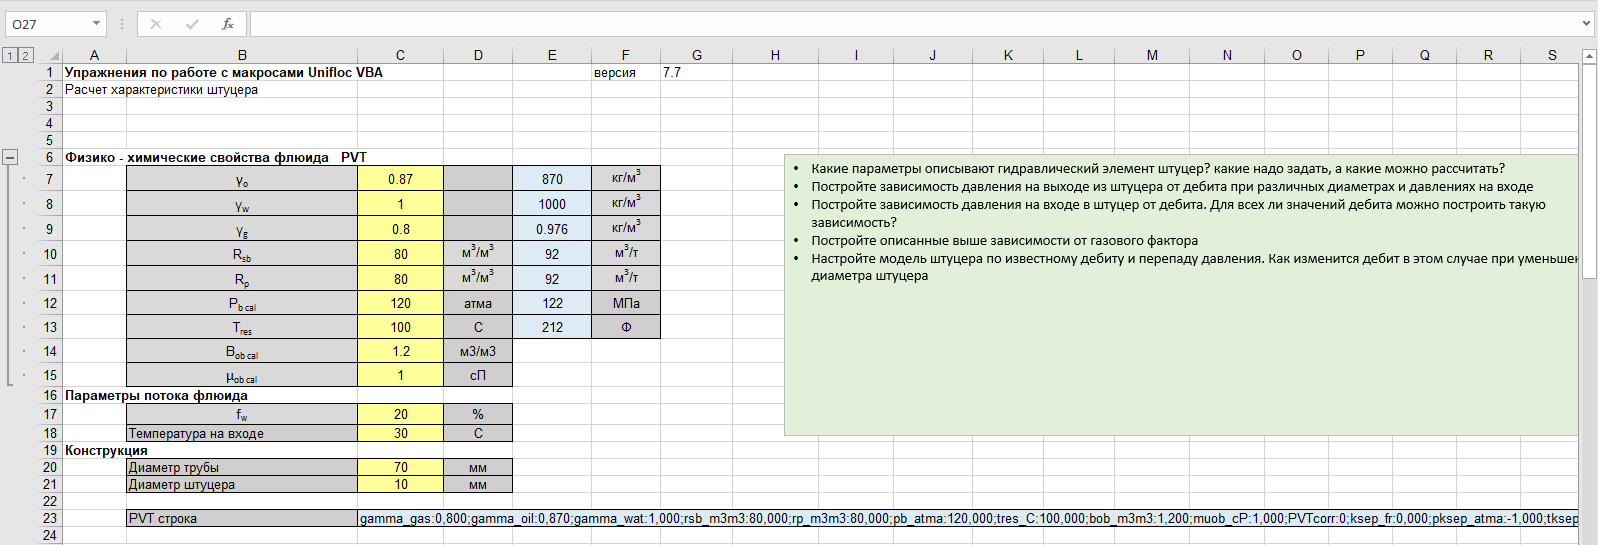
\includegraphics[width=1\linewidth]{Ex40_1}}
	\caption{Исходные данные для расчета потока через штуцер}
	\label{ris:Ex40_1}
\end{figure}

В упражнении предлагается рассчитать

\begin{enumerate}
	\item Линейное давление
	\item Буферное давление
	\item Дебит вместе с подстроечным параметром
\end{enumerate}


\begin{figure}[h!]
	\center{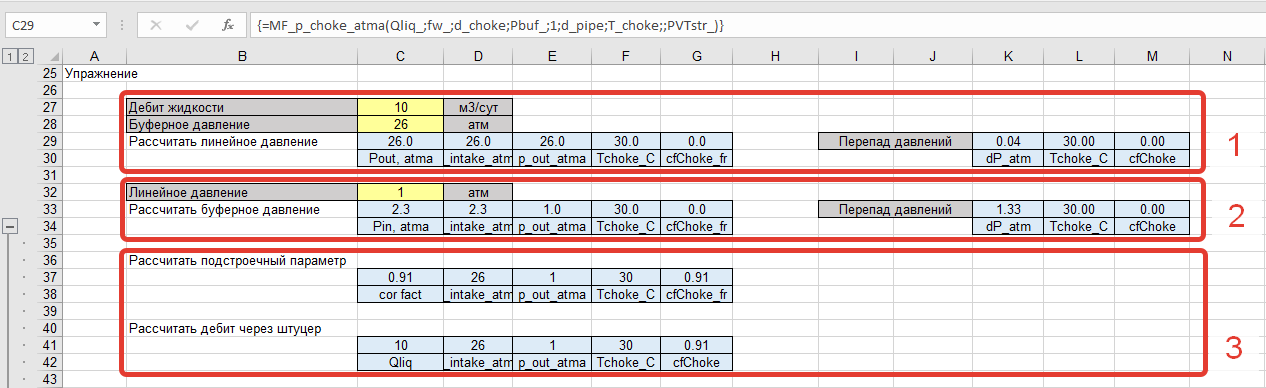
\includegraphics[width=1\linewidth]{Ex40_2}}
	\caption{Расчет давлений и дебитов через ограничитель}
	\label{ris:Ex40_2}
\end{figure}

Стоит отметить, что некоторые функции возвращают результат в виде массивов, которые занимают несколько ячеек. (Это можно определить по наличию фигурных скобок в строке формул). Поэтому для выдачи правильного результата необходимо выделить диапазон ячеек для будущего расположения массива. (Он выделен синим цветом; если диапазон окажется большим, в лишних ячейках появится сообщение "Н/Д"). После выделения диапазона наберите необходимую формулу и нажмите сочетание клавиш Ctrl+Shift+Enter.

Пользуясь инструкцией выше, для расчета линейного давления по буферному выделите диапазон C29:G30, вставьте следующую функцию в строку формул и после нажмите сочетание клавиш Ctrl+Shift+Enter.

{ \small  \texttt{=MF\_p\_choke\_atma(Qliq\_;fw\_;d\_choke;Pbuf\_;1;d\_pipe;T\_choke;;PVTstr\_)}}

Если Вы все сделали правильно, то Вы увидите массив значений из двух строк: строка названий параметров и их значения.

Аналогично для расчета перепада давления 

{ \small  \texttt{=MF\_p\_choke\_atma(Qliq\_;fw\_;d\_choke;Pbuf\_;1;d\_pipe;T\_choke;;PVTstr\_)}}

Расчет буферного давления по линейному

{ \small  \texttt{=MF\_p\_choke\_atma(Qliq\_;fw\_;d\_choke;Plin\_;0;d\_pipe;T\_choke;;PVTstr\_)
}}

И перепад давления для данного случая

{ \small  \texttt{=MF\_dp\_choke\_atm(Qliq\_;fw\_;d\_choke;Plin\_;0;d\_pipe;T\_choke;;PVTstr\_)
}}

Для вычисления дебита с помощью давлений предварительно необходимо рассчитать подстроечный параметр

{ \small  \texttt{=MF\_cf\_choke\_fr(Qliq\_;fw\_;d\_choke;Pbuf\_;Plin\_;d\_pipe;T\_choke;PVTstr\_)
}}

После возможно рассчитать уже сам дебит через штуцер

{ \small  \texttt{=MF\_qliq\_choke\_sm3day(fw\_;d\_choke;Pbuf\_;Plin\_;d\_pipe;T\_choke;C37;PVTstr\_)
}}

Чтобы построить график давления на входе штуцера от дебита при разных давлениях на выходе воспользуйтесь функцией для полного заполнения таблицы

{ \small  \texttt{=MF\_p\_choke\_atma(C\$49;fw\_;d\_choke;\$B50;0;d\_pipe;T\_choke;0;PVTstr\_)
}}


\begin{figure}[h!]
	\center{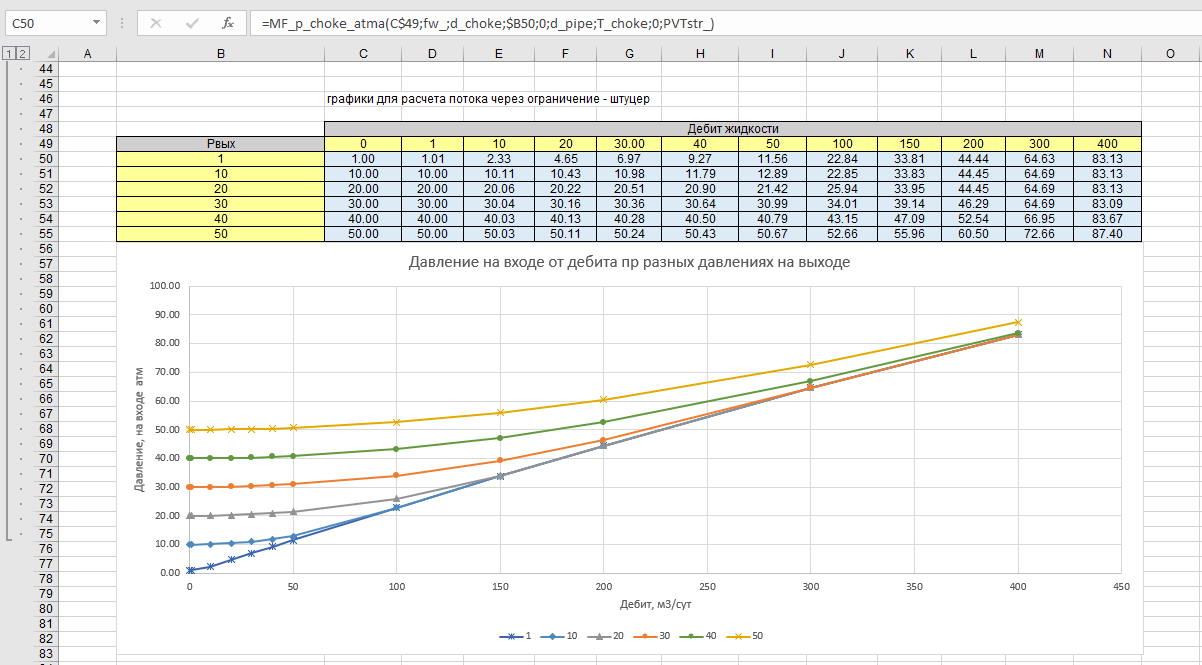
\includegraphics[width=1\linewidth]{Ex40_3}}
	\caption{Давление на входе штуцера в зависимости от различных дебитов на выходе и давлений}
	\label{ris:Ex40_3}
\end{figure}


Теперь Вы можете ответить на следующие вопросы:

\begin{enumerate}
	\item Какие параметры описывают гидравлический элемент штуцер? Какие надо задать, а какие можно рассчитать?
	\item Постройте зависимость давления на входе в штуцер от дебита. Для всех ли значений дебита можно построить такую зависимость?
	\item Настройте модель штуцера по известному дебиту и перепаду давления. Как изменится дебит в этом случае при уменьшении диаметра штуцера
\end{enumerate}




\section{Расчет распределения давления в трубе}

На распределение давления в трубе среди прочих параметров влияют режим потока газожидкостной смеси и явление проскальзывание газа. Недоучет данных параметров может привести к значительным ошибкам. Методы для расчета распределения давления можно разделить на две категории: корреляции, полученные экспериментальным путем и механистические модели, в основе которых заложены физические модели.

Для выполнение упражнения задайте PVT свойства флюидов, свойства потока и параметры трубы.

\begin{figure}[h!]
	\center{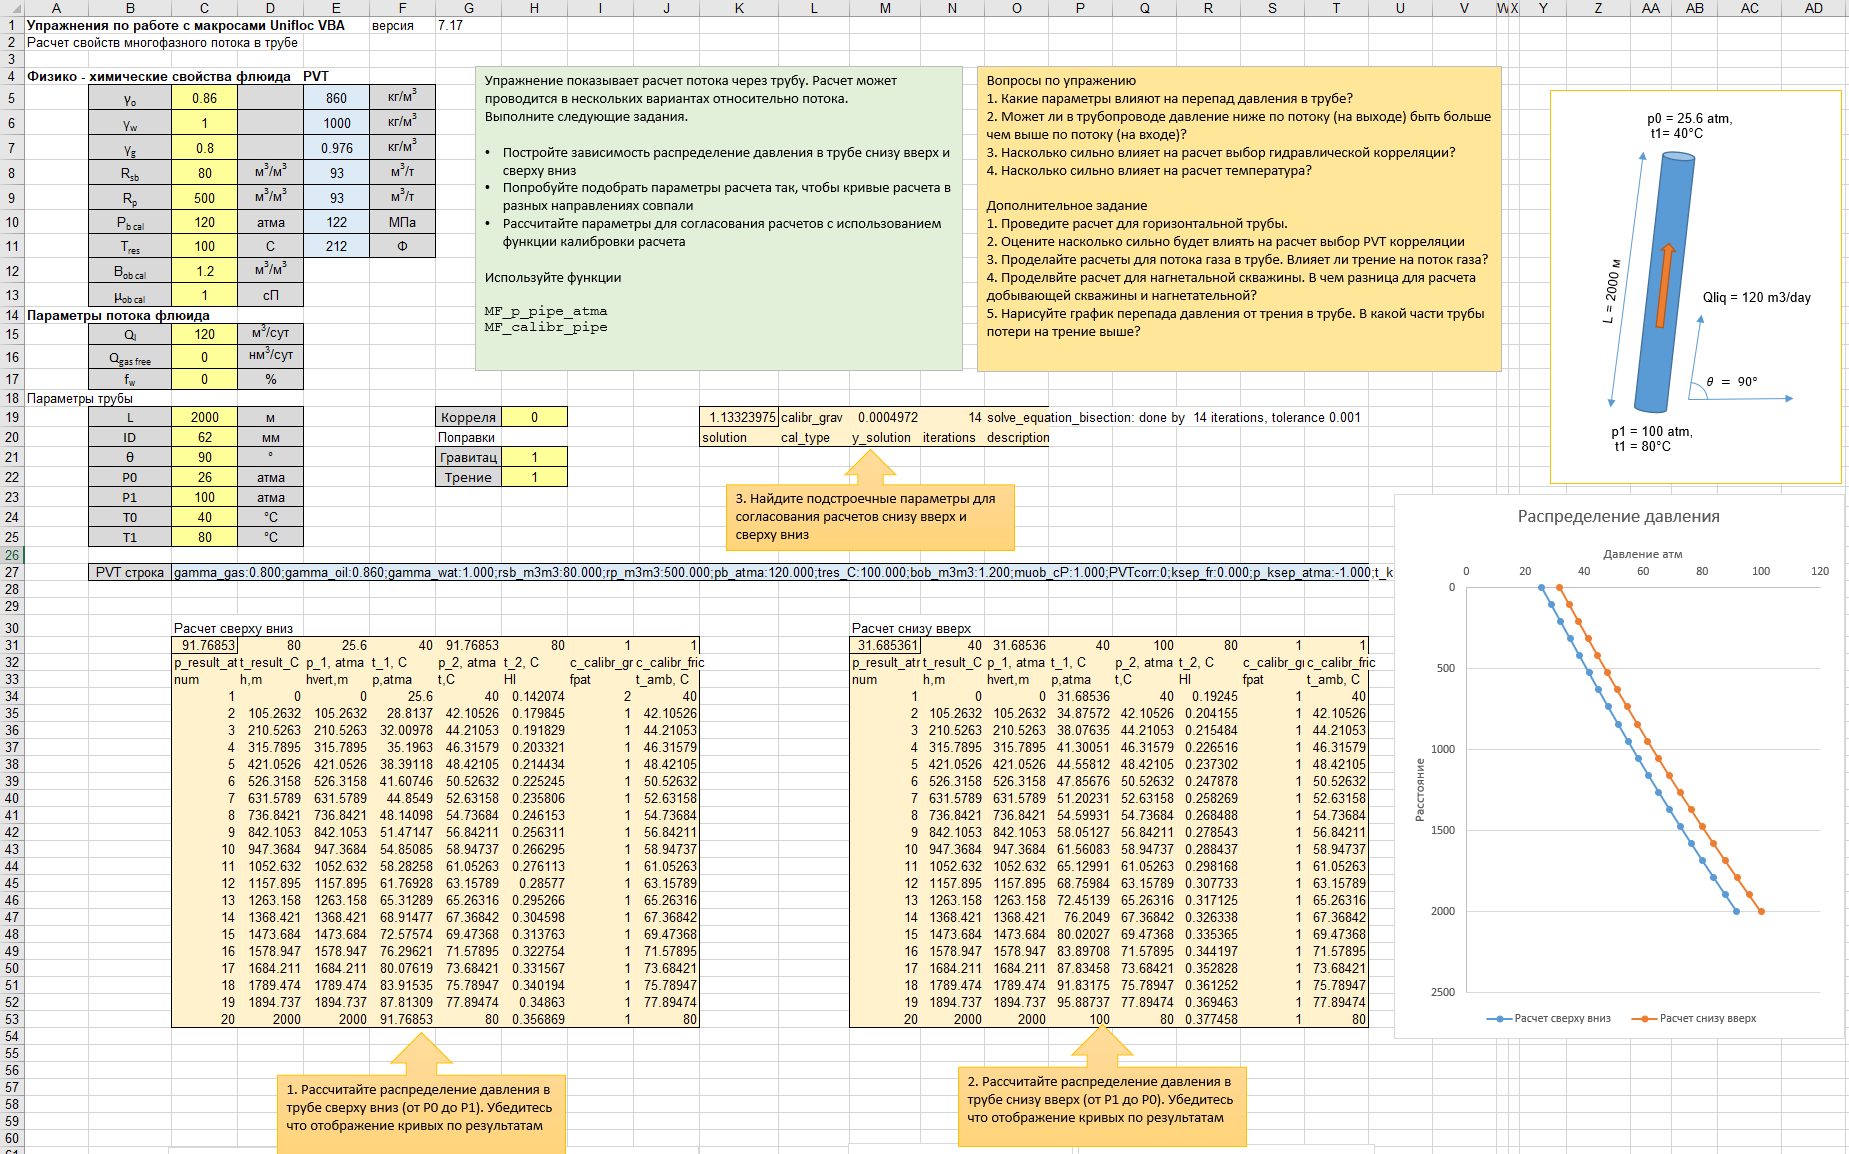
\includegraphics[width=1\linewidth]{Ex50_1}}
	\caption{Исходные данные для расчета распределения давления}
	\label{ris:Ex50_1}
\end{figure}

Где параметры трубы расшифровываются следующим образом:

$L$ - длина трубы, м

$ID$ - внутренний диаметр, мм

$\theta$ - угол наклона трубы от горизонтали, град

$P0, P1$ - давление на верхнем и нижнем конце трубы соответственно, атм

$T0, T1$  - температура на верхнем и нижнем конце трубы соответственно, С

Расчет давления в обоих направлениях ведется с помощью одной функции, возвращающий массив из 2 значений - давления и температуры. Выделите диапазон E33:F33, вставьте функцию

{ \small  \texttt{=MF\_p\_pipe\_atma(Q\_;fw\_;l0\_;C33;p0\_;PVRstr1\_;theta\_;id\_;;t0\_)
}}

и нажмите сочетание клавиш Ctrl+Shift+Enter. Далее заполните таблицу "методом протяжки"\ сверху-вниз

Обратите внимание, что расчет на каждом шаге основывается на значениях предыдущего вычисления, требуются так называемые граничные условия. 

Расчет давления снизу-вверх выполните аналогично с помощью функции, "протянув"\ ее снизу-вверх

{ \small  \texttt{=MF\_p\_pipe\_atma(Q\_;fw\_;C57;C56;G57;PVRstr1\_;theta\_;id\_;;t1\_)
}}

Для закрепления материала ответьте на вопросы

\begin{figure}[h!]
	\center{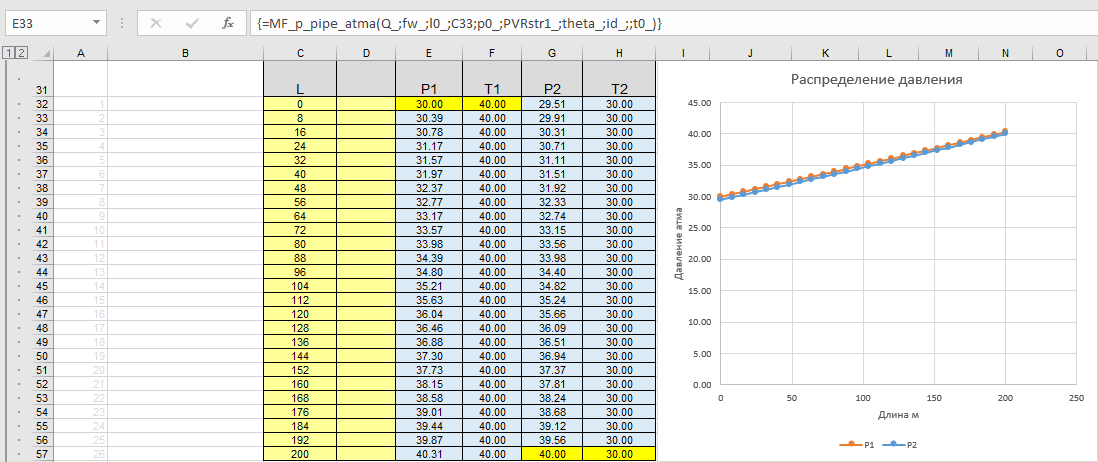
\includegraphics[width=1\linewidth]{Ex50_2}}
	\caption{Распределение давления по трубе сверху-вниз и снизу-вверх}
	\label{ris:Ex50_2}
\end{figure}

\begin{enumerate}
	\item Какие параметры влияют на перепад давления в трубе?
	\item Может ли в трубопроводе давление ниже по потоку (на выходе) быть больше чем выше по потоку (на входе)?
	\item Насколько сильно влияет на расчет выбор гидравлической корреляции PVT свойства?
	\item Насколько сильно влияет на расчет температуры давления?
\end{enumerate}

\section{Расчет коэффициентов сепарации}

Процессы сепарации на приеме погружного оборудования значительно влияют на процесс добычи. Как при естественной, так и при искусственной сепарации (при применении газосепараторов) меняются свойства многофазного потока, уменьшается газлифтный эффект, изменяется режим работы центробежного насоса.

В данном упражнении помимо стандартного определения PVT свойств требуется задать термобарические условия на приеме погружного оборудования (в месте, где происходит сепарация) и конструктивные параметры


\begin{figure}[h!]
	\center{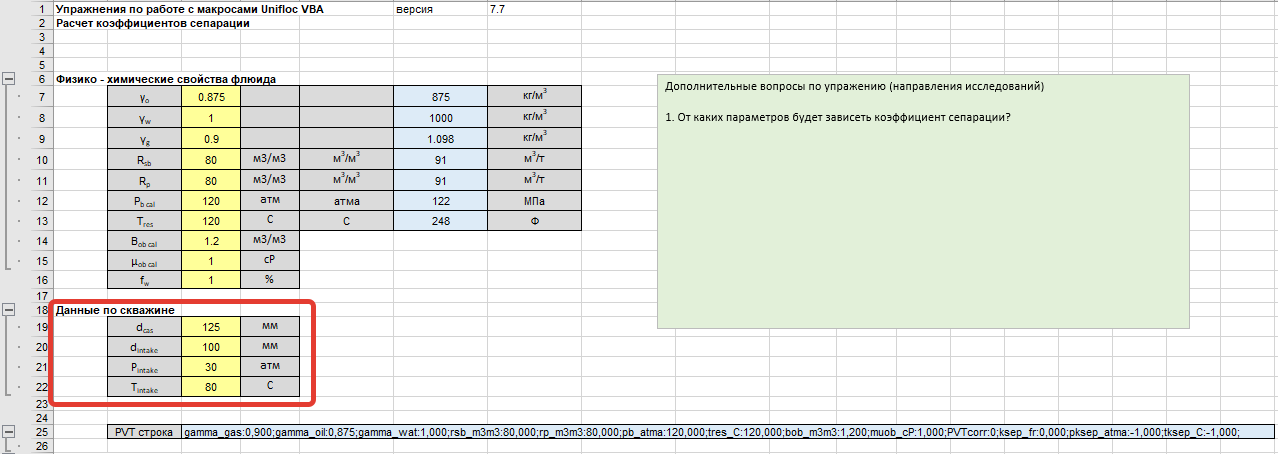
\includegraphics[width=1\linewidth]{Ex60_1}}
	\caption{Исходные данные для сепарации}
	\label{ris:Ex60_1}
\end{figure}

где

$d_{cas}$ - диаметр обсадной колонны, мм

$d_{intake}$ - диаметр приема погружного оборудования, мм

$P_{intake}$ - давление на приеме, атм

$T_{intake}$ - температура на приеме, С

Для вычисления коэффициента естественной сепарации в зависимости от дебита вставьте в ячейку E32 следующую формулу 

{ \small  \texttt{=MF\_ksep\_natural\_d(C32;wc\_;Pintake\_;Tintake\_;Dintake\_;Dcas\_;PVT\_str\_)}}

Для проведения экспериментов по влиянию изменения диаметра обсадной колонны воспользуйтесь в ячейке F32 формулой

{ \small  \texttt{=MF\_ksep\_natural\_d(C32;wc\_;Pintake\_;Tintake\_;Dintake\_;Dcas\_*cf\_dcas\_;PVT\_str\_)}}

При этом в ячейке F30 с помощью коэффициента Вы можете варьировать диаметр обсадной колонны

Для расчета доли газа в газосепараторе применяется функция

{ \small  \texttt{=MF\_gas\_fraction\_d(Pintake\_;Tintake\_;0;PVT\_str\_)*(1-F32)
}}

Коэффициент сепарации газосепаратора

{ \small  \texttt{=MF\_ksep\_gasseparator\_d(gassep\_type;G32;C32)
}}

При этом можно менять тип газосепаратора в ячейке H30

Общий коэффициент сепарации

{ \small  \texttt{=MF\_ksep\_total\_d(E32;H32)
}}

\begin{figure}[h!]
	\center{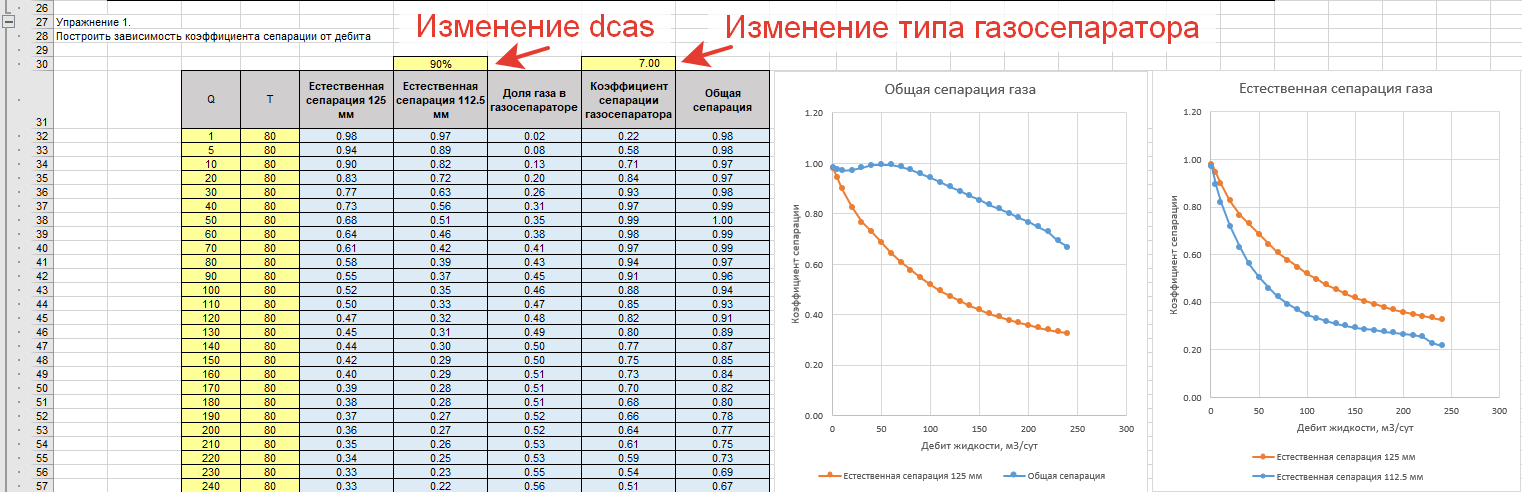
\includegraphics[width=1\linewidth]{Ex60_2}}
	\caption{Результаты расчета естественной и искусственной сепарации}
	\label{ris:Ex60_2}
\end{figure}

Вопросы к упражнению

\begin{enumerate}
	\item От каких параметров будет зависеть коэффициент сепарации?
	\item Как взаимосвязана естественная и искусственная сепарация? 
\end{enumerate}


\section{Анализ работы ЭЦН}

Сегодня доминирующая доля нефти в РФ добывается при помощи ЭЦН. Требуется детальное понимание основных особенностях эксплуатации данного оборудования, режимах работы, возможных осложнениях по причине высокой вязкости продукции, газосодержания, механических примесей и т.д.

Наиболее ценную информацию о работе насоса может дать его характеристика: зависимость параметров работы ЭЦН - напора, потребляемой мощности, перепада давления, КПД, от подачи (дебита скважины)

Для анализа работы скважины, оснащенной УЭЦН, требуются следующие исходные данные

\begin{enumerate}
	\item Физико - химические свойства флюида
	\item Данные по скважине
	\item Данные по ЭЦН
	\item Параметры пласта
\end{enumerate}

PVT свойства задаются аналогично предыдущим упражнениям, а для параметров, характеризующих скважину, приняты следующие обозначения

$H_{mes}$ - глубина скважины измеренная (вдоль ствола скважины), м

$H_{mes}- H_{vert}$ - удлинение ствола скважины, м

$H_{pump}$ - глубина спуска насоса, м

$ID_{cas}$ - внутренний диаметр обсадной колонны, мм

$OD_{tub}$ - внешний диаметр НКТ, мм

$ID_{tub}$ - внутренний диаметр НКТ, мм

$D_{intake}$ - диаметр приемной сетки ЭЦН, мм

$P_{buf}$ - буферное давление, атм

$P_{intake}$ - давление на приеме ЭЦН, атм

$T_{intake}$ - температура на приеме ЭЦН, С

$P_{dis}$ - давление на выкиде ЭЦН, атм

$P_{wf}$ - давление на забое, атм

$Q_{liq}$ - дебит жидкости в поверхностных условиях, м3/сут

$f_w$ - обводненность в поверхностных условиях, \%

\begin{figure}[h!]
	\center{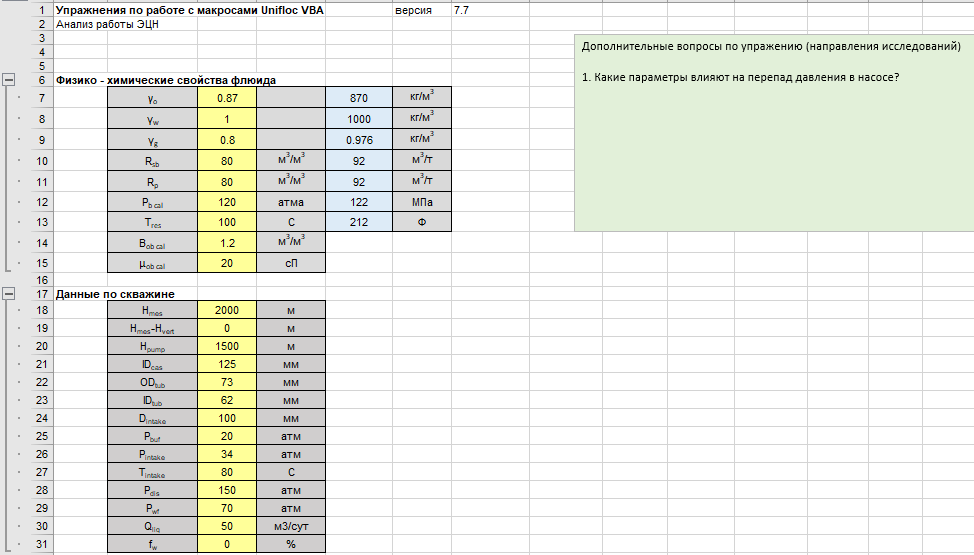
\includegraphics[width=1\linewidth]{Ex70_1}}
	\caption{Исходные данные для свойств флюида и параметров скважины}
	\label{ris:Ex70_1}
\end{figure}

Параметры, описывающие ЭЦН: 

ЭЦН $Q_{nom}$ - номинальная подача ЭЦН, м3/сут

ЭЦН $H_{nom}$ - номинальная напом ЭЦН, м

$F$ - частота питающего тока двигателя, Гц

ЭЦН $ID$ - идентификационный номер насоса (по формуле, см. ниже), находящийся в базе \unf

ЭЦН имя - обозначение насоса: название, габарит и номинальная подача (по формуле, см. ниже)

ЭЦН $Q_{max}$ - максимальная производительность насоса (по формуле, см. ниже), м3/сут

Ступени - количество ступеней, исходя из общего напора ЭЦН и напора одной ступени (по формуле, см. ниже), шт

$K_{sep_ГС}$ - коэффициент сепарации газосепаратора, \%

$P_{sep}$ - давление сепарации, атм

$T_{sep}$ - температура сепарации, С

Данные о пласте:

$P_{res}$ - пластовое давление, атм

$PI$ - коэффициент продуктивности скважины (по формуле, см. выше в упражнении IPR), м3/сут/атм

$\frac{dT}{dL}$ - геотермический градиент, град / 100 м

\begin{figure}[h!]
	\center{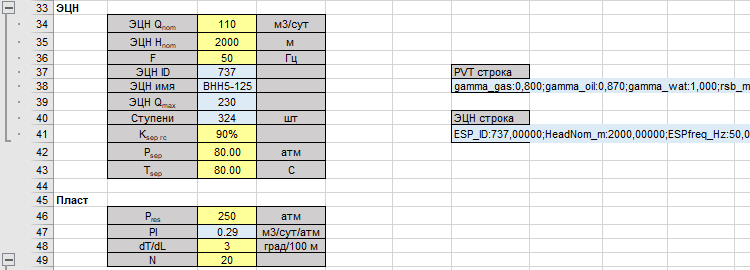
\includegraphics[width=1\linewidth]{Ex70_2}}
	\caption{Исходные данные для ЭЦН и пласта}
	\label{ris:Ex70_2}
\end{figure}

Для получения идентификационного номера насоса в базе \unf \ была использована формула

{ \small  \texttt{=ESP\_id\_by\_rate(Q\_ESP\_)}}

Для определения обозначения ЭЦН

{ \small  \texttt{=ESP\_name(C37)}}

Расчет максимально возможного дебита

{ \small  \texttt{=esp\_max\_rate\_m3day(Freq\_;PumpID\_)*1}}

Количество ступеней

{ \small  \texttt{=ЦЕЛОЕ(Head\_ESP\_/ESP\_head\_m(Q\_ESP\_;1;;PumpID\_))
}}

Также для удобства использования параметры насоса: ID, напор и рабочая частота, зашифровываются в строку с помощью функции

{ \small  \texttt{=ESP\_Encode\_string(PumpID\_;Head\_ESP\_;Freq\_)}}

Свободный газ негативно влияет на работу ЭЦН. В ячейке D51 вычисляется объемная доля газа на приеме газосепаратора с помощью формулы

{ \small  \texttt{=MF\_gas\_fraction\_d(Pintake\_;Tintake\_;fw\_;PVTstr)}}
 
В соседней ячейке D50 для удобного расположения задается вязкость в сПуаз

Построение напорной характеристики данного насоса выполняется с учетом вязкости перекачиваемой продукции. Реализованный метод пересчета характеристики с воды на вязкую жидкость Института Гидравлики позволяет учитывать изменение рабочих параметров из-за данного негативного влияния.

Для вычисления напора в метрах водного столба в ячейке D54 воспользуйтесь формулой

{ \small  \texttt{=ESP\_head\_m(C54;NumStage\_;Freq\_;PumpID\_;mu)}}

КПД ЭЦН в долях единиц 

{ \small  \texttt{=ESP\_eff\_fr(C54;NumStage\_;Freq\_;PumpID\_;mu)}}

Потребляемую ЭЦН мощность в Вт

{ \small  \texttt{=ESP\_Power\_W(C54;NumStage\_;Freq\_;PumpID\_;mu)}}

\begin{figure}[h!]
	\center{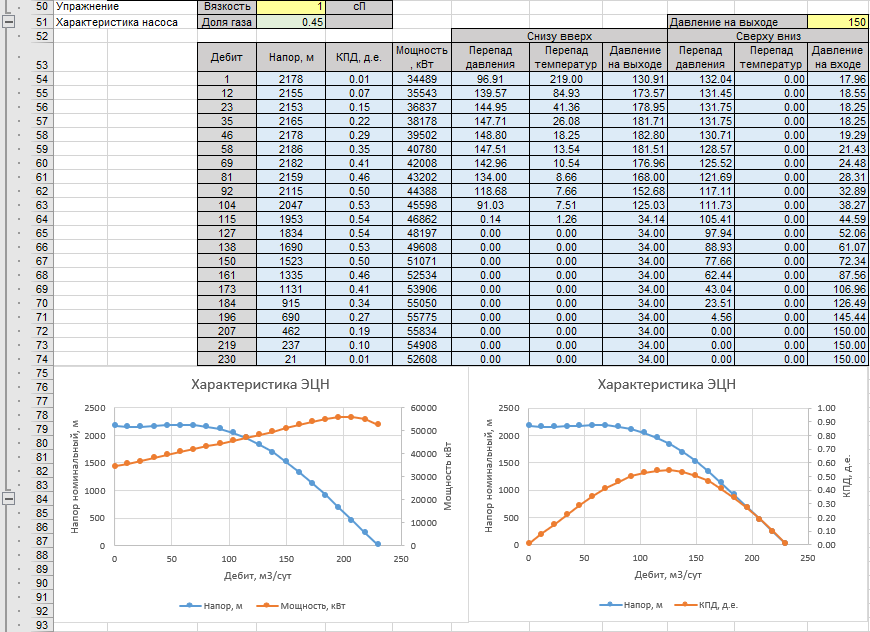
\includegraphics[width=1\linewidth]{Ex70_3}}
	\caption{Напорные характеристики ЭЦН с поправкой на вязкость}
	\label{ris:Ex70_3}
\end{figure}

Расчет перепада давления, развиваемого насосом, может происходить методом "сверху-вниз" \  и "снизу-вверх" \ , при этом расчет перепада температур только методом "снизу-вверх". Функция расчета перепада давления и температуры возвращает массив значений, т.е. одновременно перепад давления и температуры. Кроме того, входным параметром для данной функции является направление расчета. Для вычисления выделите диапазон G54:H54, наберите формулу

{ \small  \texttt{=ESP\_dP\_atm(C54;fw\_;Pintake\_;NumStage\_;Freq\_;PumpID\_;PVTstr;Tintake\_;0)}}

и после нажмите сочетание клавиш  Ctrl+Shift+Enter. Далее протяните результат до полного заполнения двух столбцов.

Зная давление на приеме и перепад давления в ЭЦН, давление на выходе ЭЦН можно легко посчитать по формуле

{ \small  \texttt{=G54+Pintake\_}}

Предварительно задав давление на выходе ЭЦН в ячейке L51 возможно посчитать перепад давления методом "сверху-вниз"\ аналогичным образом по формуле

{ \small  \texttt{=ESP\_dP\_atm(C54;fw\_;Pdis\_;NumStage\_;Freq\_;PumpID\_;PVTstr;Tintake\_;Tintake\_;0)}}

И давление на входе, зная давление на выходе и перепад давления

{ \small  \texttt{=Pdis-J54}}

\begin{figure}[h!]
	\center{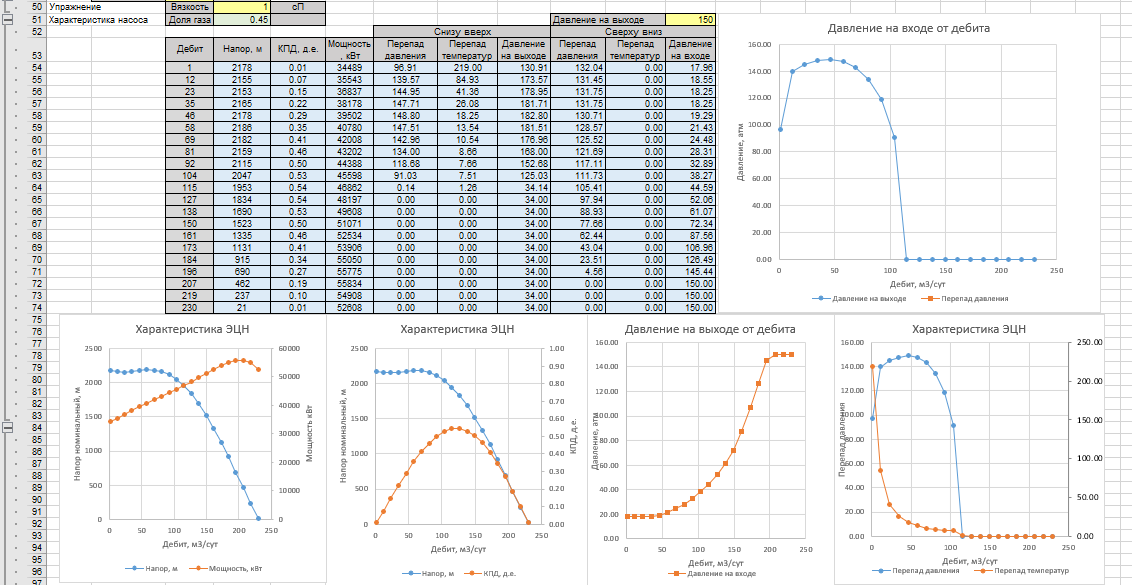
\includegraphics[width=1\linewidth]{Ex70_4}}
	\caption{Расчет перепада давления и температур в ЭЦН в зависимости от дебита}
	\label{ris:Ex70_4}
\end{figure}

Вопросы для упражнения:

\begin{enumerate}
	\item Какие параметры влияют на перепад давления в насосе?
	\item Насколько сильно влияет вязкость на напорные характерситики ЭЦН?
	\item Как влияет на работу ЭЦН изменение частоты?
\end{enumerate}


\section{Анализ работы ПЭД}

Упражнение показывает характеристики погружного асинхронного электрического двигателя, применяемого в УЭЦН.

Также стоит отметить, что расчетные функции предназначаются для образовательных целей. Детального сопоставления расчетных характеристик с фактическими не проводилось. (06.2019)

Для выполнения упражнения необходимо задать параметры электродвигателя

$U_{nom}$ - номинальное напряжение ПЭД, В

$F_{nom}$ - номинальная частота тока, Гц

$I_{nom}$ - номинальная сила тока, А

$ID$ - способ инициализации данных двигателя. 1 - по фактическим значениям параметров (по паспорту), 2 - по схеме замещения Гридина

А также рабочее напряжение $U$, В и рабочую частоту тока $F$, Гц

После этого в ячейке С10 будет произведен расчет номинальной мощности ПЭД с помощью функции

{ \small  \texttt{=Motor\_Pnom\_kW(Unom;Inom;Fnom;ID)}}

\begin{figure}[h!]
	\center{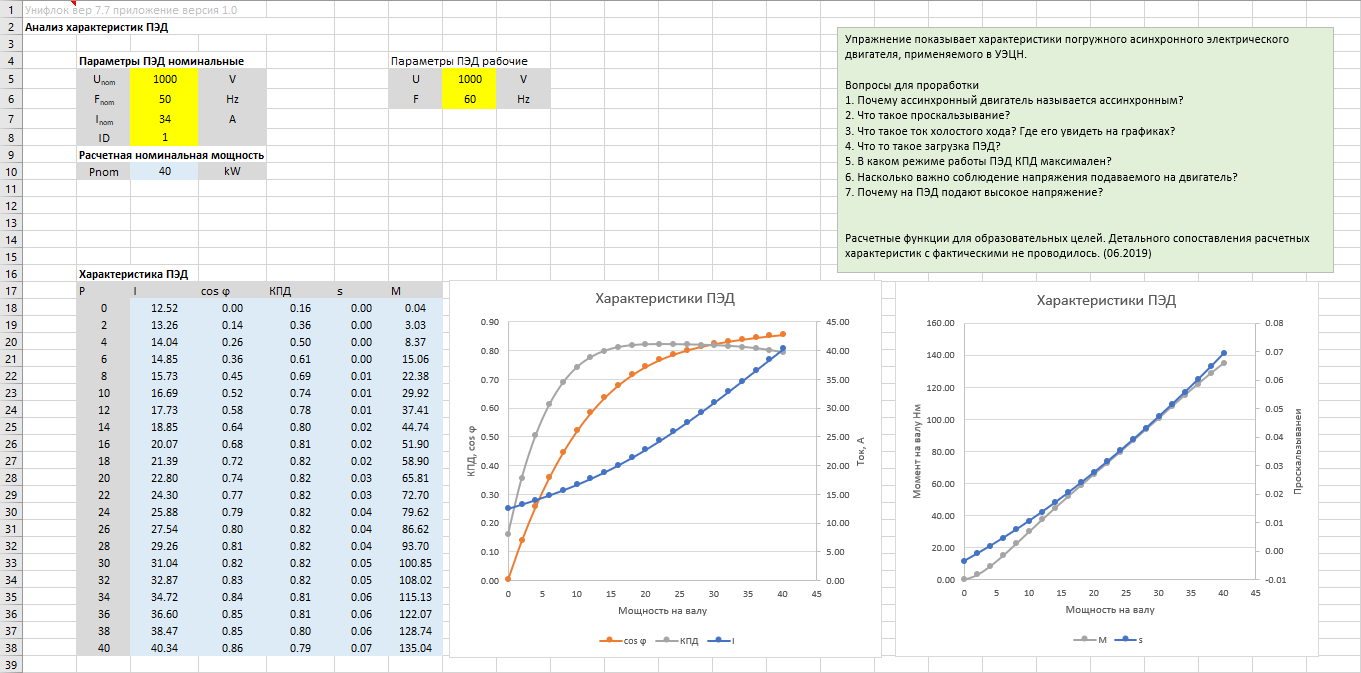
\includegraphics[width=1\linewidth]{Ex80_1}}
	\caption{Исходные данные ПЭД и различные характеристики в зависимости от мощности на валу}
	\label{ris:Ex80_1}
\end{figure}

Для построения характеристики ПЭД (параметры двигателя от мощности на валу $M$) воспользуйтесь следующими формулами

Определение тока двигателя $I$, A

{ \small  \texttt{=motor\_I\_A(B18;F;U;Unom;Inom;Fnom;ID)}}

Расчет $cos \varphi $

{ \small  \texttt{=motor\_CosPhi\_d(B18;F;U;Unom;Inom;Fnom;ID)}}

КПД, д.ед.

{ \small  \texttt{=motor\_Eff\_d(B18;F;U;Unom;Inom;Fnom;ID)}}

Проскальзывание $S$

{ \small  \texttt{=motor\_S\_d(B18;F;U;Unom;Inom;Fnom;ID)}}

Момент на валу $M$, Н*м

{ \small  \texttt{=motor\_M\_Nm(B18;F;U;Unom;Inom;Fnom;ID)}}

\begin{figure}[h!]
	\center{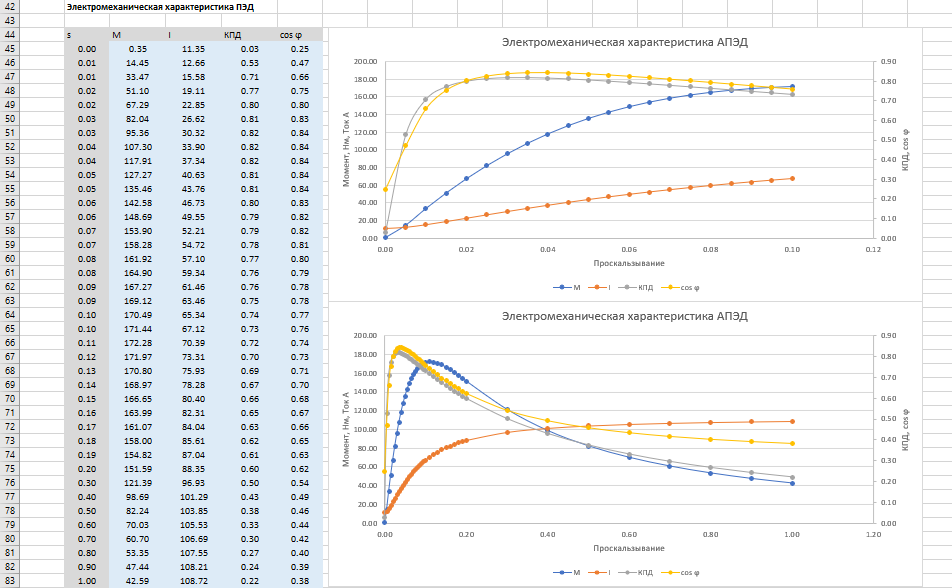
\includegraphics[width=1\linewidth]{Ex80_2}}
	\caption{Электромеханическая характеристика АПЭД}
	\label{ris:Ex80_2}
\end{figure}

Для расчета электромеханической характеристики АПЭД (параметры двигателя в зависимости от проскальзывания $S$) используйте формулы

Момент на валу $M$, Н*м 

{ \small  \texttt{=motor\_M\_slip\_Nm(B45;F;U;Unom;Inom;Fnom;0)}}

Сила тока $I$, А

{ \small  \texttt{=motor\_I\_slip\_A(B45;F;U;Unom;Inom;Fnom;0)}}

КПД, д.ед.

{ \small  \texttt{=motor\_Eff\_slip(B45;F;U;Unom;Inom;Fnom;0)}}

Расчет $cos \varphi $

{ \small  \texttt{=motor\_CosPhi\_slip(B45;F;U;Unom;Inom;Fnom;0)}}


\begin{figure}[h!]
	\center{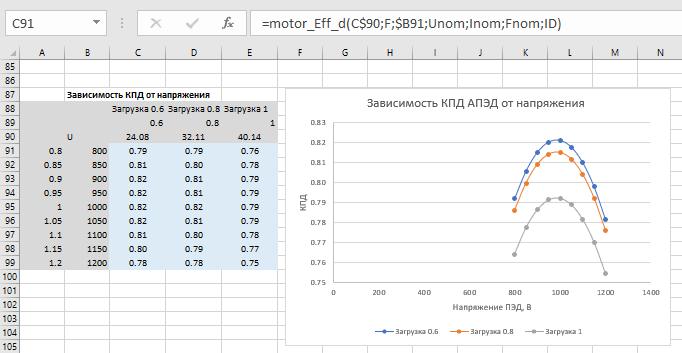
\includegraphics[width=1\linewidth]{Ex80_3}}
	\caption{Зависимость КПД АПЭД от напряжения и загрузки}
	\label{ris:Ex80_3}
\end{figure}

Для проведения исследований по напряжению ПЭД воспользуйтесь следующими формулами для значений загрузки двигателя 0.6, 0.8, 1 

{ \small  \texttt{=motor\_Eff\_d(C\$90;F;\$B91;Unom;Inom;Fnom;ID)}}

{ \small  \texttt{=motor\_Eff\_d(D\$90;F;\$B91;Unom;Inom;Fnom;ID)}}

{ \small  \texttt{=motor\_Eff\_d(E\$90;F;\$B91;Unom;Inom;Fnom;ID)}}

в ячейках C91, E91, D91 соответственно. "Протянув"\ значения Вы можете заполнить таблицу.

Вопросы для упражнения:

\begin{enumerate}
	\item Почему ассинхронный двигатель называется ассинхронным?
	\item Что такое проскальзывание?
	\item Что такое ток холостого хода? Где его увидеть на графиках?
	\item Что то такое загрузка ПЭД?
	\item В каком режиме работы ПЭД КПД максимален?
	\item Насколько важно соблюдение напряжения подаваемого на двигатель?
	\item Почему на ПЭД подают высокое напряжение?
\end{enumerate}


\section{Набор расчетных модулей анализа скважины}
Пример использования алгоритмов \unf   приведен в файле \texttt{UF7\_calc\_well.xlsm}.

Файл содержит набор расчетных модулей позволяющих провести анализ данных описывающих работу скважины с применением различных методов добычи.

\subsection{Расчетный модуль анализа и настройки PVT свойств}

